% Options for packages loaded elsewhere
% Options for packages loaded elsewhere
\PassOptionsToPackage{unicode}{hyperref}
\PassOptionsToPackage{hyphens}{url}
\PassOptionsToPackage{dvipsnames,svgnames,x11names}{xcolor}
%
\documentclass[
  british,
  a4paper,
]{article}
\usepackage{xcolor}
\usepackage{amsmath,amssymb}
\setcounter{secnumdepth}{-\maxdimen} % remove section numbering
\usepackage{iftex}
\ifPDFTeX
  \usepackage[T1]{fontenc}
  \usepackage[utf8]{inputenc}
  \usepackage{textcomp} % provide euro and other symbols
\else % if luatex or xetex
  \usepackage{unicode-math} % this also loads fontspec
  \defaultfontfeatures{Scale=MatchLowercase}
  \defaultfontfeatures[\rmfamily]{Ligatures=TeX,Scale=1}
\fi
\usepackage{lmodern}
\ifPDFTeX\else
  % xetex/luatex font selection
\fi
% Use upquote if available, for straight quotes in verbatim environments
\IfFileExists{upquote.sty}{\usepackage{upquote}}{}
\IfFileExists{microtype.sty}{% use microtype if available
  \usepackage[]{microtype}
  \UseMicrotypeSet[protrusion]{basicmath} % disable protrusion for tt fonts
}{}
\makeatletter
\@ifundefined{KOMAClassName}{% if non-KOMA class
  \IfFileExists{parskip.sty}{%
    \usepackage{parskip}
  }{% else
    \setlength{\parindent}{0pt}
    \setlength{\parskip}{6pt plus 2pt minus 1pt}}
}{% if KOMA class
  \KOMAoptions{parskip=half}}
\makeatother
% Make \paragraph and \subparagraph free-standing
\makeatletter
\ifx\paragraph\undefined\else
  \let\oldparagraph\paragraph
  \renewcommand{\paragraph}{
    \@ifstar
      \xxxParagraphStar
      \xxxParagraphNoStar
  }
  \newcommand{\xxxParagraphStar}[1]{\oldparagraph*{#1}\mbox{}}
  \newcommand{\xxxParagraphNoStar}[1]{\oldparagraph{#1}\mbox{}}
\fi
\ifx\subparagraph\undefined\else
  \let\oldsubparagraph\subparagraph
  \renewcommand{\subparagraph}{
    \@ifstar
      \xxxSubParagraphStar
      \xxxSubParagraphNoStar
  }
  \newcommand{\xxxSubParagraphStar}[1]{\oldsubparagraph*{#1}\mbox{}}
  \newcommand{\xxxSubParagraphNoStar}[1]{\oldsubparagraph{#1}\mbox{}}
\fi
\makeatother


\usepackage{longtable,booktabs,array}
\newcounter{none} % for unnumbered tables
\usepackage{calc} % for calculating minipage widths
% Correct order of tables after \paragraph or \subparagraph
\usepackage{etoolbox}
\makeatletter
\patchcmd\longtable{\par}{\if@noskipsec\mbox{}\fi\par}{}{}
\makeatother
% Allow footnotes in longtable head/foot
\IfFileExists{footnotehyper.sty}{\usepackage{footnotehyper}}{\usepackage{footnote}}
\makesavenoteenv{longtable}
\usepackage{graphicx}
\makeatletter
\newsavebox\pandoc@box
\newcommand*\pandocbounded[1]{% scales image to fit in text height/width
  \sbox\pandoc@box{#1}%
  \Gscale@div\@tempa{\textheight}{\dimexpr\ht\pandoc@box+\dp\pandoc@box\relax}%
  \Gscale@div\@tempb{\linewidth}{\wd\pandoc@box}%
  \ifdim\@tempb\p@<\@tempa\p@\let\@tempa\@tempb\fi% select the smaller of both
  \ifdim\@tempa\p@<\p@\scalebox{\@tempa}{\usebox\pandoc@box}%
  \else\usebox{\pandoc@box}%
  \fi%
}
% Set default figure placement to htbp
\def\fps@figure{htbp}
\makeatother



\ifLuaTeX
\usepackage[bidi=basic,shorthands=off]{babel}
\else
\usepackage[bidi=default,shorthands=off]{babel}
\fi
\ifLuaTeX
  \usepackage{selnolig} % disable illegal ligatures
\fi


\setlength{\emergencystretch}{3em} % prevent overfull lines

\providecommand{\tightlist}{%
  \setlength{\itemsep}{0pt}\setlength{\parskip}{0pt}}



 


\makeatletter
\@ifpackageloaded{tcolorbox}{}{\usepackage[skins,breakable]{tcolorbox}}
\@ifpackageloaded{fontawesome5}{}{\usepackage{fontawesome5}}
\definecolor{quarto-callout-color}{HTML}{909090}
\definecolor{quarto-callout-note-color}{HTML}{0758E5}
\definecolor{quarto-callout-important-color}{HTML}{CC1914}
\definecolor{quarto-callout-warning-color}{HTML}{EB9113}
\definecolor{quarto-callout-tip-color}{HTML}{00A047}
\definecolor{quarto-callout-caution-color}{HTML}{FC5300}
\definecolor{quarto-callout-color-frame}{HTML}{acacac}
\definecolor{quarto-callout-note-color-frame}{HTML}{4582ec}
\definecolor{quarto-callout-important-color-frame}{HTML}{d9534f}
\definecolor{quarto-callout-warning-color-frame}{HTML}{f0ad4e}
\definecolor{quarto-callout-tip-color-frame}{HTML}{02b875}
\definecolor{quarto-callout-caution-color-frame}{HTML}{fd7e14}
\makeatother
\makeatletter
\@ifpackageloaded{caption}{}{\usepackage{caption}}
\AtBeginDocument{%
\ifdefined\contentsname
  \renewcommand*\contentsname{Table of contents}
\else
  \newcommand\contentsname{Table of contents}
\fi
\ifdefined\listfigurename
  \renewcommand*\listfigurename{List of Figures}
\else
  \newcommand\listfigurename{List of Figures}
\fi
\ifdefined\listtablename
  \renewcommand*\listtablename{List of Tables}
\else
  \newcommand\listtablename{List of Tables}
\fi
\ifdefined\figurename
  \renewcommand*\figurename{Figure}
\else
  \newcommand\figurename{Figure}
\fi
\ifdefined\tablename
  \renewcommand*\tablename{Table}
\else
  \newcommand\tablename{Table}
\fi
}
\@ifpackageloaded{float}{}{\usepackage{float}}
\floatstyle{ruled}
\@ifundefined{c@chapter}{\newfloat{codelisting}{h}{lop}}{\newfloat{codelisting}{h}{lop}[chapter]}
\floatname{codelisting}{Listing}
\newcommand*\listoflistings{\listof{codelisting}{List of Listings}}
\makeatother
\makeatletter
\makeatother
\makeatletter
\@ifpackageloaded{caption}{}{\usepackage{caption}}
\@ifpackageloaded{subcaption}{}{\usepackage{subcaption}}
\makeatother
\usepackage{bookmark}
\IfFileExists{xurl.sty}{\usepackage{xurl}}{} % add URL line breaks if available
\urlstyle{same}
% fallback for those not using the hyperref driver hyperxmp:
\makeatletter
\@ifundefined{xmpquote}{\newcommand{\xmpquote}[1]{#1}}{}
\makeatother
\hypersetup{
  pdftitle={Combining forecasting methods is the robust choice},
  pdfauthor={Carlos Galindo},
  pdflang={en-GB},
  colorlinks=true,
  linkcolor={blue},
  filecolor={Maroon},
  citecolor={Blue},
  urlcolor={Blue},
  pdfcreator={LaTeX via pandoc}}


\title{Combining forecasting methods is the robust choice}
\usepackage{etoolbox}
\makeatletter
\providecommand{\subtitle}[1]{% add subtitle to \maketitle
  \apptocmd{\@title}{\par {\large #1 \par}}{}{}
}
\makeatother
\subtitle{Across 181 US consumer-price components, the leading method
shifts from component to component and month to month, and a simple
average of the methods is the most accurate forecast over the full test
year}
\author{Carlos Galindo}
\date{}
\begin{document}
\maketitle


\begin{tcolorbox}[enhanced jigsaw, arc=.35mm, bottomrule=.15mm, breakable, colback=white, colframe=quarto-callout-note-color-frame, left=2mm, leftrule=.75mm, opacityback=0, rightrule=.15mm, toprule=.15mm]

\vspace{-3mm}\textbf{At a glance}\vspace{3mm}

\begin{itemize}
\tightlist
\item
  \textbf{Question.} Which forecasting method should a bottom-up
  inflation forecaster rely on for each part of the US consumer-price
  index, and how stable is that choice?
\item
  \textbf{Approach.} Eight methods from different model families, and
  their simple average, compete on 181 price components in twelve
  rolling one-month-ahead tests over the most recent year, each scored
  against a naive benchmark.
\item
  \textbf{Finding.} Leadership is spread across methods and shifts from
  month to month. The simple average is the most accurate forecast over
  the full test year and the one entry that improves on the naive
  benchmark. For the typical component, every method improves on it.
\item
  \textbf{Why it matters.} When no method leads consistently, combining
  them gives the stability of the group rather than the risk of a single
  choice. The average is cheap to compute and is the natural default for
  a component-level forecasting system.
\end{itemize}

\end{tcolorbox}

\subsection{The question}\label{the-question}

Forecasters who work from the bottom up, building headline inflation
from its components, face a practical problem. A consumer-price index
has well over a hundred published components, and they do not behave
alike. Rents move slowly. Energy and some food items swing sharply.
Apparel and travel carry strong seasonal patterns and large one-off
spikes. A method that suits one of these may not suit another.

The usual answer is to pick a method and apply it everywhere, or to pick
the best method for each component after some testing. Both rest on the
assumption that there is a stable winner to find. This project tests
that assumption directly. For each component, and in each of a sequence
of monthly tests, which method is best, how large is its edge over a
naive forecast, and is the edge stable enough to rely on?

\subsection{Approach}\label{approach}

\textbf{Coverage.} The comparison covers 181 components of the US
consumer price index for all urban consumers, from the broad headline
down to detailed items.

\textbf{Candidate methods.} Nine forecasts compete on every component:
eight individual methods and their simple, equally weighted average. The
individual methods are statistical models of different families. Some
forecast the underlying trend and seasonal pattern of the series
directly, others split the series into trend, seasonal and irregular
parts and forecast each part separately, and one treats the irregular
spikes explicitly. All are built to run automatically, so that the same
procedure applies to every component without hand tuning.

\textbf{Scoring.} Each forecast is scored by its mean absolute error,
scaled by the mean absolute one-period change of the series itself. This
is the mean absolute scaled error. A score of 1 means the method matches
the naive benchmark, which assumes the series simply carries on from
where it is. A score below 1 means it improves on that benchmark.
Scaling by the series' own volatility puts a calm item like rent and a
volatile one like fuel on the same footing, so averages across
components are meaningful.

\textbf{Rolling tests.} Scores come from twelve rolling out-of-sample
tests over the most recent year. For each of the twelve most recent
months in turn, the sample is cut just before that month, every model is
re-estimated on the data up to that point, and its one-month-ahead
forecast is scored against the published outcome. Each component
therefore receives twelve one-month-ahead tests, one per month of the
test year, and no forecast is judged on data it has seen.

\textbf{Combination.} Beyond the simple average, the pipeline also
includes weights that favour methods with lower past error, using an
exponential decay of the scaled error, normalised to sum to one. The
comparison reported here uses the equal-weight average.

\subsection{What the work shows}\label{what-the-work-shows}

\textbf{Leadership is spread across methods.} Across the 181 components,
the method that comes first most often does so for 38, about one
component in five. Leadership also shifts from test to test. In the most
recent test month the most frequent leader is first for 32 components,
while in the test seven months back a different method leads, for 40.

\textbf{Lasting leadership is the exception.} Only six components have a
method that leads in six or more of the twelve tests, and the longest
such run is ten. For the others, leadership moves between methods from
one test month to another.

\textbf{The average is the most accurate forecast over the full year.}
Across all twelve tests, the simple average scores 0.989 on the scaled
error: the lowest of the nine entries, and below the naive benchmark of
1. The individual methods score between 1.04 and 1.33. The margin is
narrow, and that is informative in itself: monthly price components
carry little predictable signal beyond their recent past, so improving
on the naive benchmark across 181 components and a full year is
demanding, and the average does so.

\begin{figure}

\centering{

\pandocbounded{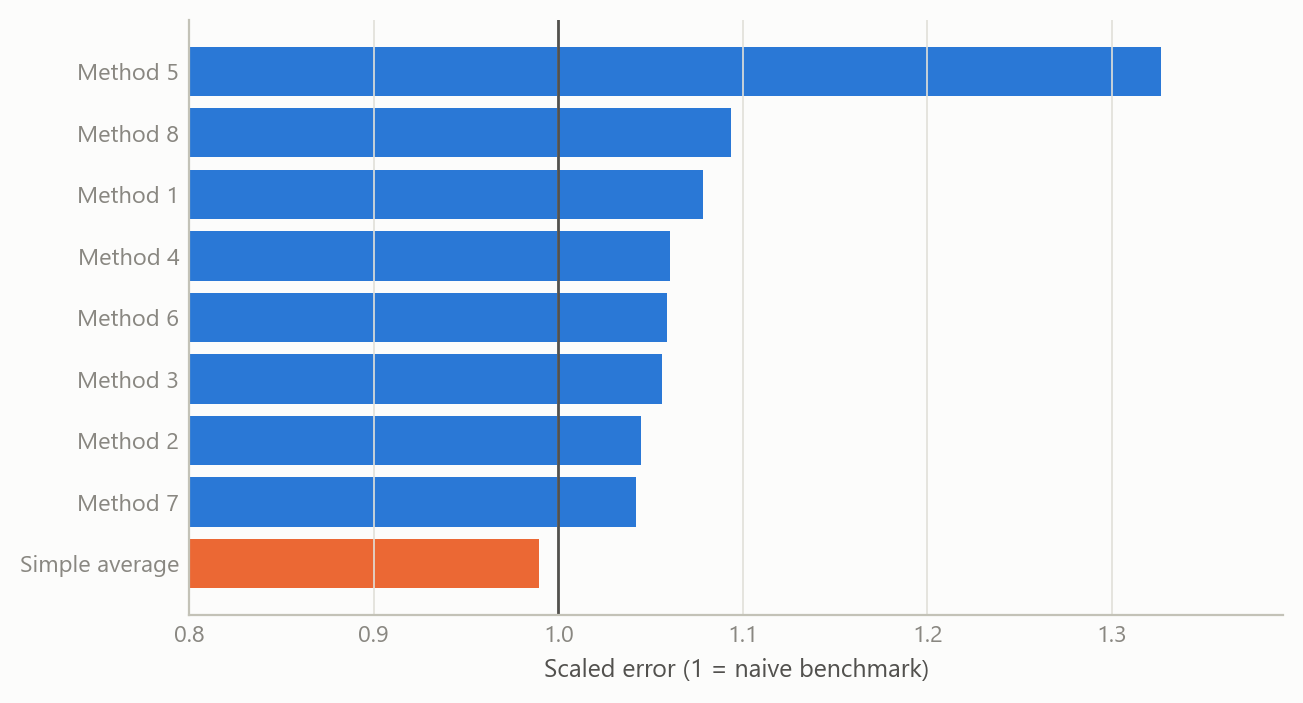
\includegraphics[keepaspectratio]{index_files/figure-latex/fig-mase-output-1.png}}

}

\caption{\label{fig-mase}Mean scaled error over all twelve tests and 181
components, by method, against the naive benchmark at 1.0. Source:
summary results of the comparison (September 2025); author's
calculations.}

\end{figure}%

\textbf{Month by month, the average is most often the best.} In an
October 2025 re-run of the comparison on the same 181 components, the
simple average has the lowest mean error in six of the twelve test
months, and in a seventh it is a close second (0.8633 against 0.8631).
No individual method is lowest in more than one test month.

\textbf{The typical component is forecast well.} In the same re-run, the
median component's scaled error is below 1 for every method in every
test month, at most 0.86. Mean errors sit near 1 because a minority of
components carry large errors. Those components are where
series-specific attention is most likely to pay off.

\begin{figure}

\centering{

\pandocbounded{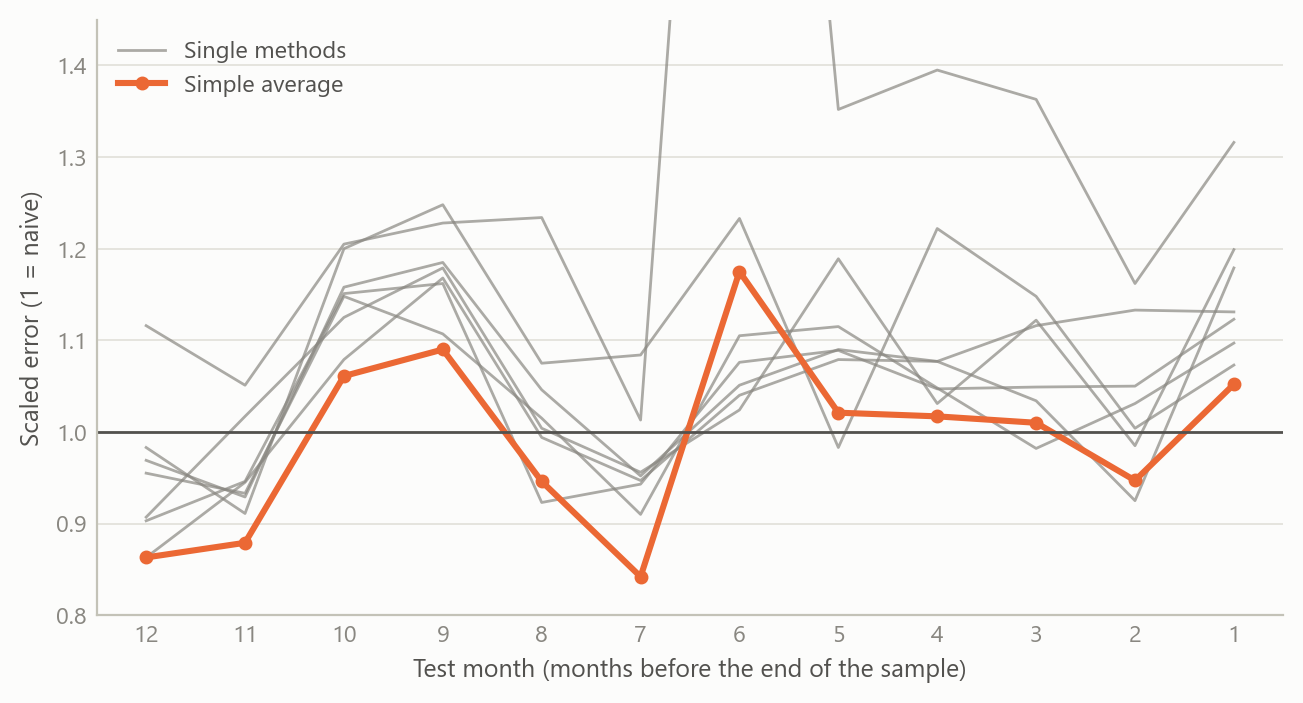
\includegraphics[keepaspectratio]{index_files/figure-latex/fig-tests-output-1.png}}

}

\caption{\label{fig-tests}Mean scaled error in each of the twelve
one-month-ahead tests, 181 components, against the naive benchmark at
1.0. Grey: the single methods; orange: their simple average. Tests run
from twelve months before the end of the sample (left) to one month
before (right). One method reaches 2.48 in the test six months back,
above the top of the scale. Source: October 2025 re-run of the
comparison (seven distinct methods); author's calculations.}

\end{figure}%

The last two figures are simulated to share the shape of the exercise,
with the same components, the same twelve test months and the same eight
methods plus an average. They show the mechanism, not measured numbers.

\begin{figure}

\centering{

\pandocbounded{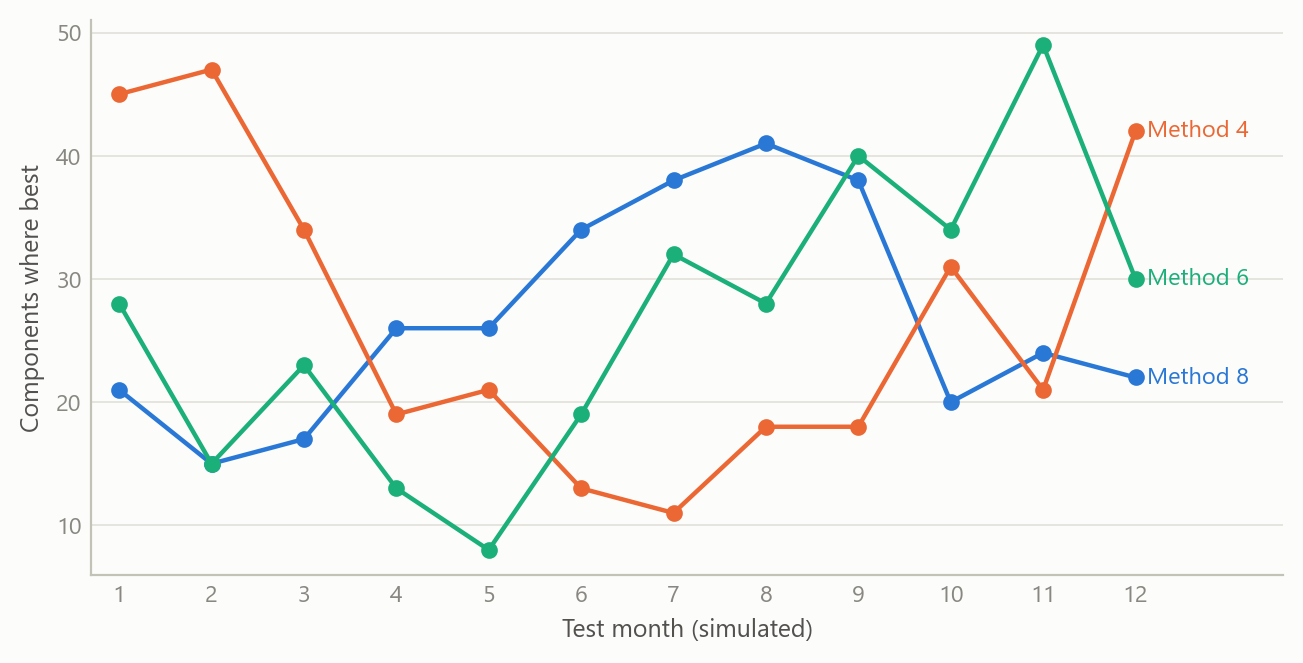
\includegraphics[keepaspectratio]{index_files/figure-latex/fig-leaders-output-1.png}}

}

\caption{\label{fig-leaders}Number of components for which each of three
methods is best, test by test (simulated data).}

\end{figure}%

Each line is one method's count of component wins. The lines cross, so
the ranking in one test month is not the ranking in the next.

\subsection{Insights}\label{insights}

\begin{enumerate}
\def\labelenumi{\arabic{enumi}.}
\tightlist
\item
  \textbf{Combining is insurance against a shifting leader.} When the
  best method changes with the component and with the month, a choice
  made on past results is a bet that leadership persists. Averaging
  gives up the chance of being exactly right in return for protection
  against being badly wrong, and over the full year that trade pays.
\item
  \textbf{The naive benchmark is the right yardstick.} For monthly price
  components, ``no change from here'' is a demanding standard. Scoring
  every method against it, rather than against other models, shows
  directly whether a forecast adds information.
\item
  \textbf{Scale the error, then average across components.} Without
  scaling by each series' own volatility, the volatile components
  dominate any average. The scaled error makes the comparison fair
  across rent, energy and apparel.
\item
  \textbf{Every method has a place.} The method with the weakest overall
  score still leads for some components and test months. Judging methods
  only by their overall average hides where each one adds value, which
  is an argument for combining rather than culling.
\item
  \textbf{Hard cases show where to specialise.} A small set of
  components is hard for the automated methods, and on some of them the
  weighting gives certain methods zero weight. These cases mark where a
  series-specific approach adds most.
\end{enumerate}

\begin{figure}

\centering{

\pandocbounded{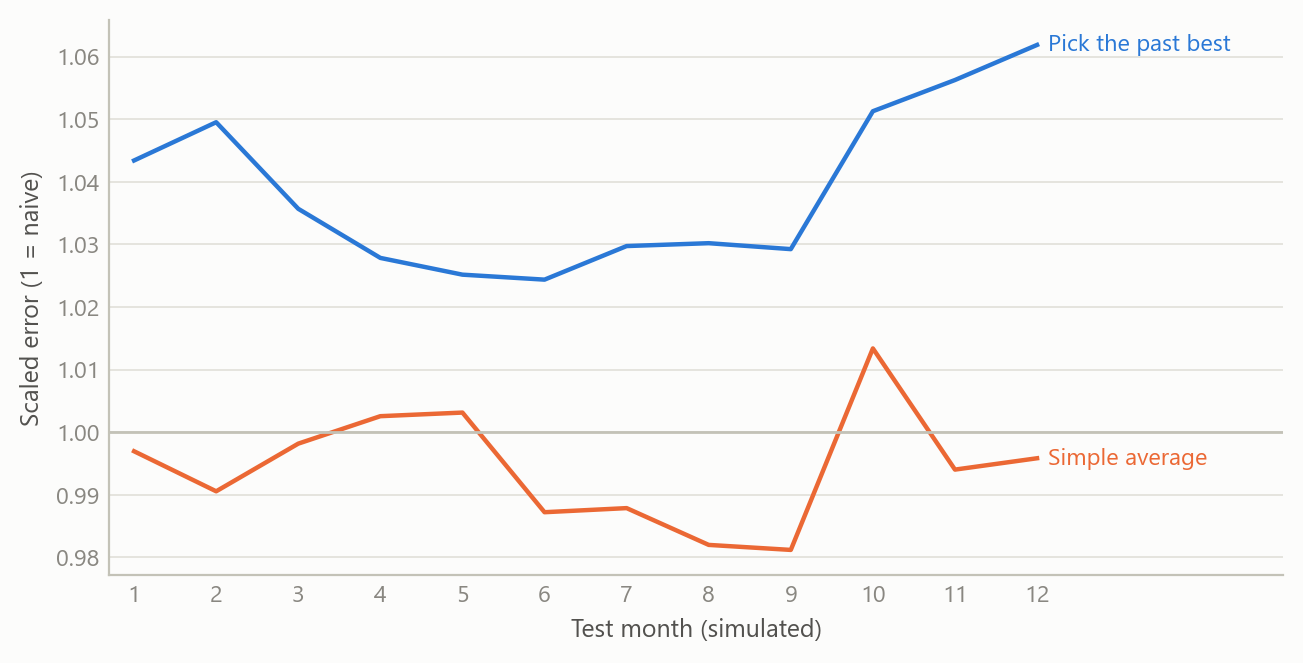
\includegraphics[keepaspectratio]{index_files/figure-latex/fig-select-output-1.png}}

}

\caption{\label{fig-select}Out-of-sample scaled error test by test:
choosing the best past method per component versus the simple average
(simulated data).}

\end{figure}%

This figure illustrates insight 1. A method chosen because it won a
first round tends to do worse on the next round than the average of all
of them, because part of its win was luck. It is a simulation of that
mechanism and does not report a measured gap.

\subsection{Scope and next steps}\label{scope-and-next-steps}

\begin{itemize}
\tightlist
\item
  \textbf{Selection versus averaging, measured.} The stored
  month-by-month scores allow a direct out-of-sample test of insight 1:
  choose each component's method on the earlier test months and judge it
  on the later ones, against the average.
\item
  \textbf{Size of the margin.} A formal test of forecast accuracy across
  many series, with a correction for multiple comparisons, would show
  how much of the average's full-year margin over the benchmark is
  systematic.
\item
  \textbf{Counts and magnitudes.} Win counts show how often a method
  leads. The month-by-month profile above adds how far each method is
  from the benchmark.
\item
  \textbf{Weighted combinations.} Evaluating the error-based weights
  against the equal-weight average on held-out months is a natural
  extension.
\item
  \textbf{Wider coverage.} The comparison covers US consumer prices over
  a recent year that includes unusual inflation. Repeating it across
  economies and over calmer periods would show how general the result
  is.
\end{itemize}

\subsection{About the evidence}\label{about-the-evidence}

The comparison is real: 181 US consumer-price components, twelve rolling
one-month-ahead tests over the most recent year, completed in 2025 as
part of the rebuild of a forecasting pipeline during a career break. The
overall scores and leader counts come from its summary results
(September 2025), and the month-by-month profile comes from an October
2025 re-run of the same comparison. The first two figures show measured
results. The last two are simulated.

Figures and tables marked \emph{simulated} are generated from simulated
data built to share the structure of the analysis (its variables,
horizons and frequencies). They show how each method works and what its
output looks like. Results stated in the text, and figures that give a
source, are the project's own. Methods are described at the level of a
methods section. Code and data pipelines are not reproduced here.




\end{document}
